
%%%%%%%%%%% Nomenclature for this chapter%%%%%%%%%%
\nomenclature{TAU}{Tel-Aviv University}
%%%%%%%%%%%%%%%%%%%%%%%%%%%%%%%%%%%%


\chapter{Basic examples}
\label{chap:chapter 1}

This paper is wonderful \cite{kour2014real}.
See Figure \ref{fig:figure_label} and Table \ref{table:table_ex}.\\

\begin{figure}
\centering
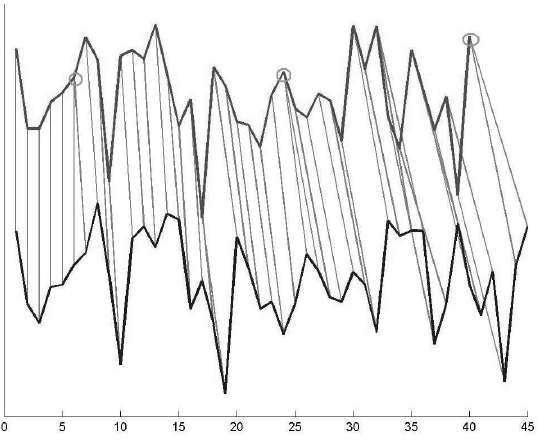
\includegraphics[width=0.5\textwidth]{./figures/figure}
\caption{A figure example.}
\label{fig:figure_label}
\end{figure}

\section{Section 1}
\label{sec:section1}

\begin{table}
\centering
\caption{A table example}
\begin{tabular}{ c c c c }
\toprule
\textbf{Dataset} & \textbf{Number of samples} & \textbf{Results} & \textbf{Results 2} \\
\midrule                 
  Ini & 1405 & 48 & 9 \\ 
  Mid & 1196 & 52 & 10 \\ 
  Fin & 1629 & 44 & 9 \\ 
  Iso & 1372 & 39 & 8 \\ 
  \bottomrule
\end{tabular}
\label{table:table_ex} 
\end{table}



\section {Nomenclature}

For updating nomenclature run the following commands:

makeindex Thesis-main.nlo -s nomencl.ist -o Thesis-main.nls

makeindex LettersClassification.nlo -s nomencl.ist -o LettersClassification.